\documentclass{article}

% NeurIPS 2025 style. Use [preprint] for arXiv/preprint (authors shown, no
% line numbers); switch to [main] for a double-blind submission or
% [main, final] for the camera-ready.
\usepackage[preprint]{neurips_2025}

\usepackage[utf8]{inputenc}
\usepackage[T1]{fontenc}
\usepackage{amsmath,amssymb,amsthm}
\usepackage{graphicx}
\usepackage{booktabs}
\usepackage{multirow}
\usepackage[ruled,vlined]{algorithm2e}
\usepackage{float}
\usepackage{pifont}
\usepackage{tikz}
\usetikzlibrary{positioning,fit,arrows.meta,backgrounds,calc}
\usepackage{microtype}
\usepackage{xcolor}
\usepackage{hyperref}

% Float placement: pack figures/tables tightly and allow them near their
% reference, so pages don't end up half blank and text stays next to the
% figure it discusses.
\renewcommand{\topfraction}{0.92}
\renewcommand{\bottomfraction}{0.85}
\renewcommand{\textfraction}{0.08}
\renewcommand{\floatpagefraction}{0.72}
\setcounter{topnumber}{3}
\setcounter{bottomnumber}{2}
\setcounter{totalnumber}{5}

\newcommand{\shortclosepct}{97\%}
\newcommand{\truncgapmax}{1.38}
\newcommand{\klreduxfactor}{44.2$\times$}
\newcommand{\beyondgain}{0.024}
\newcommand{\beyondheadroom}{0.061}
\newcommand{\beyondgainpct}{39\%}
\newcommand{\certmarginmin}{0.03}
\newcommand{\certmarginmax}{1.30}
\newcommand{\chunkonekl}{0.019}
\newcommand{\chunkfivekl}{0.283}


\newcommand{\Dtot}{D_{\mathrm{tot}}}
\newcommand{\Dfar}{D'}
\newcommand{\Dloc}{D}
\newcommand{\KL}[2]{\mathrm{KL}\!\left(#1 \,\middle\|\, #2\right)}
\newcommand{\rep}{\mathrm{rep}}
\newtheorem{proposition}{Proposition}
\newtheorem{remark}{Remark}
\newcommand{\cmark}{\ding{51}}
\newcommand{\xmark}{\ding{55}}

\title{LongRange-PFN: KL-Distilled Recursive Latent Summaries\\
for Prior-Fitted Networks beyond the Context Window}

\author{%
  Antonio J.~Brych\thanks{Correspondence: \texttt{abrych@arborcapital.com.br}} \\
  FGV EMAp \\
  \And
  Gabriel Abad \\
  FGV EMAp \\
}

\begin{document}
\maketitle

\begin{abstract}
Prior-fitted networks (PFNs) return a Bayesian posterior in one forward pass,
but only up to the context size seen in training: attention is quadratic and
quality drops past that window. LongRange-PFN compresses the distant context
$\Dfar$ into $k$ latent tokens $z = \rep(\Dfar)$ with a learned summarizer, and
predicts from the local context $\Dloc$ with $z$ added as extra tokens. We
distill a frozen full-context teacher PFN by matching predictive
distributions; since both use the same discretized output, the KL is exact. A
recursive summarizer $z_t = \rep(C_t, z_{t-1})$ folds the distant context one
chunk at a time at constant state, so inference is not capped by the training
window. On Gaussian-process priors, where the true posterior is known, the
student's NLL falls \certmarginmin--\certmarginmax{} nats below a lower bound
available to any method that sees only $\Dloc$, closing \shortclosepct{} of the
truncation gap; and in a streaming setting at $4\times$ the training window the
recursive summary beats a teacher restricted to the most recent points,
recovering $\approx\beyondgainpct{}$ of the remaining headroom. We also report
where it fails: multi-chunk summarization trails single-shot, and bounded-state
inference still loses to classical full-context baselines on this easy prior.
\end{abstract}

\section{Introduction}
\label{sec:intro}

Prior-fitted networks \citep{muller2022pfn} treat Bayesian prediction as
in-context learning: pre-train a transformer on data sets drawn from a prior,
then at test time feed it a training set $\Dtot$ and a query $x$ and read off an
approximation to $p(y \mid x, \Dtot)$. TabPFN
\citep{hollmann2023tabpfn, hollmann2025tabpfn} made this a practical tabular
model. But the context is the model's memory: every observation is a token,
attention is $O(|\Dtot|^2)$, and the network never saw contexts larger than
some $N$ in training. Past $N$ it faces a cost problem and a distribution
shift, and the usual fix, subsampling $\Dtot$, discards likelihood terms and
provably widens the posterior.

Existing approaches (Section~\ref{sec:related}) optimize a compact context per
data set at test time \citep{feuer2024tunetables, ma2024icd}, retrieve real
neighbors \citep{thomas2024localpfn}, or, in language models, compress prompts
into soft tokens \citep{mu2023gisting, ge2023icae, chevalier2023autocompressors}.
None gives a PFN a fixed-size, reusable summary of what the far-away data
contributed to the posterior.

LongRange-PFN splits $\Dtot = \Dfar \cup \Dloc$, compresses $\Dfar$ into $k$
latent tokens $z = \rep_\phi(\Dfar)$ with a learned summarizer (one forward
pass, no test-time optimization), and predicts from $[\,z \mid \Dloc \mid x\,]$
with a standard PFN backbone that treats $z$ as ordinary context. Training
distills a frozen full-context teacher PFN: teacher and student share the same
discretized (``bar'') output, so the KL between their predictions is an exact
categorical KL with no sampling. The summarizer is recursive,
$z_t = \rep_\phi(C_t, z_{t-1})$: it folds a stream of chunks into a fixed-size
summary, mirroring the Bayesian filtering update
$p(\rho \mid C_{1:t}) \propto p(C_t \mid \rho)\, p(\rho \mid C_{1:t-1})$ over a
latent task $\rho$. This decouples how much data the system uses from the
window any component was trained on: distilled only on contexts of at most
$80$ points and $3$ chunks, the model still handles $320$ points in five chunks
at inference, beating a strong recency baseline (Table~\ref{tab:beyond}).

\paragraph{Contributions.}
\begin{enumerate}
  \item A summary-conditioned PFN trained by exact predictive KL distillation
  (Section~\ref{sec:method}): $\rep_\phi(\Dfar)$ is learned end-to-end so that
  $q_\phi(y \mid x, \Dloc, z)$ matches a frozen teacher's
  $p_\theta(y \mid x, \Dtot)$, with an exact bucket-level KL.
  \item A recursive summary update (Section~\ref{sec:recursive}) giving
  bounded-state PFN inference beyond the pre-training window, to our knowledge
  the first such mechanism for PFNs.
  \item Validation against the exact GP posterior
  (Section~\ref{sec:experiments}), including a lower bound the student provably
  crosses, plus an honest account of what still fails.
\end{enumerate}

\begin{figure}[htbp]
\centering
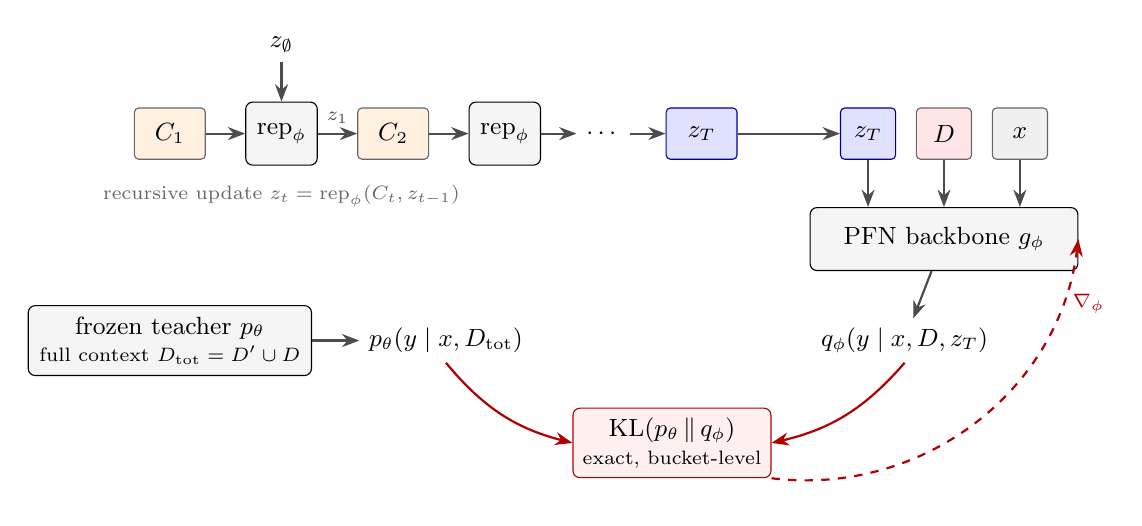
\begin{tikzpicture}[
  font=\small,
  chunk/.style={draw=black!60, fill=orange!12, rounded corners=1.5pt,
    minimum width=9mm, minimum height=6.5mm, inner sep=1.5pt},
  ztok/.style={draw=blue!60!black, fill=blue!12, rounded corners=1.5pt,
    minimum width=9mm, minimum height=6.5mm, inner sep=1.5pt},
  module/.style={draw=black, fill=black!4, rounded corners=2.5pt,
    minimum height=8mm, inner sep=4pt, align=center},
  loss/.style={draw=red!70!black, fill=red!6, rounded corners=2.5pt,
    minimum height=7mm, inner sep=3.5pt, align=center},
  arr/.style={-{Stealth[length=2.2mm]}, thick, black!70},
]
\node[chunk] (c1) {$C_1$};
\node[module, right=5mm of c1] (rep1) {$\rep_\phi$};
\node[chunk, right=5mm of rep1] (c2) {$C_2$};
\node[module, right=5mm of c2] (rep2) {$\rep_\phi$};
\node[right=4.5mm of rep2] (dots) {$\cdots$};
\node[ztok, right=4.5mm of dots] (zT) {$z_T$};
\node[above=5mm of rep1] (z0) {$z_\emptyset$};
\draw[arr] (z0) -- (rep1);
\draw[arr] (c1) -- (rep1);
\draw[arr] (rep1) -- node[above, font=\scriptsize] {$z_1$} (c2.west |- rep1.east);
\draw[arr] (c2) -- (rep2);
\draw[arr] (rep2) -- (dots);
\draw[arr] (dots) -- (zT);
\node[below=1.2mm of rep1.south, font=\scriptsize, black!60] {recursive update
  $z_t = \rep_\phi(C_t, z_{t-1})$};

\node[ztok, right=13mm of zT, minimum width=7mm] (zin) {$z_T$};
\node[chunk, fill=red!10, right=2.5mm of zin, minimum width=7mm] (dloc) {$\Dloc$};
\node[chunk, fill=black!6, right=2.5mm of dloc, minimum width=7mm] (xq) {$x$};
\node[module, below=6mm of dloc, minimum width=34mm] (backbone)
  {PFN backbone $g_\phi$};
\draw[arr] (zT) -- (zin);
\draw[arr] (zin.south) -- (backbone.north -| zin.south);
\draw[arr] (dloc.south) -- (backbone.north -| dloc.south);
\draw[arr] (xq.south) -- (backbone.north -| xq.south);
\node[below=6mm of backbone, xshift=-5mm, align=center] (q)
  {$q_\phi(y \mid x, \Dloc, z_T)$};
\draw[arr] (backbone) -- (q);

\node[module, align=center] (teacher) at (c1 |- q)
  {frozen teacher $p_\theta$\\[-1pt]{\scriptsize full context $\Dtot = \Dfar \cup \Dloc$}};
\node[right=6mm of teacher, align=center] (p) {$p_\theta(y \mid x, \Dtot)$};
\draw[arr] (teacher) -- (p);
\node[loss] (kl) at ($($(p.east)!0.5!(q.west)$)+(0,-13mm)$)
  {$\mathrm{KL}(p_\theta \,\Vert\, q_\phi)$\\[-1pt]{\scriptsize exact, bucket-level}};
\draw[arr, red!70!black] (p.south) to[bend right=18] (kl.west);
\draw[arr, red!70!black] (q.south) to[bend left=18] (kl.east);
\draw[arr, red!70!black, dashed] (kl.south east) to[bend right=45]
  node[right, pos=0.85, font=\scriptsize, red!70!black] {$\nabla_\phi$}
  (backbone.east);
\end{tikzpicture}
\caption{\textbf{LongRange-PFN.} $\Dfar$ streams through the summarizer in
chunks; the recursive update keeps an $O(k)$ state (left). The backbone
predicts from $[\,z_T \mid \Dloc \mid x\,]$, treating summary tokens as context
(right). Training minimizes the exact bucket-level KL to a frozen full-context
teacher (bottom); no ground-truth posterior is needed.}
\label{fig:schematic}
\end{figure}

\section{Background}
\label{sec:background}

\paragraph{PFNs approximate the posterior.} Let $p(\rho)$ be a prior over tasks
and $p(\mathcal{D} \mid \rho)$ a likelihood over data sets. A PFN $p_\theta$ is
trained by sampling $\mathcal{D} \sim p(\mathcal{D})$, splitting it into a
context $\Dtot$ and queries $(x, y)$, and minimizing
$\mathbb{E}[-\log p_\theta(y \mid x, \Dtot)]$. \citet{muller2022pfn} show this
minimizes the expected KL to the true posterior predictive up to a constant, so
the minimizer is
\begin{equation}
\label{eq:ppd}
  p(y \mid x, \Dtot) \;=\; \int p(y \mid x, \rho)\; p(\rho \mid \Dtot)\, d\rho .
\end{equation}
For regression, $p_\theta$ outputs a \emph{bar distribution}: a
piecewise-constant density over $B$ buckets with borders fixed from prior
quantiles.

\paragraph{The window problem.} Let $N$ be the largest context length seen in
training. For $|\Dtot| > N$ a PFN faces $O(|\Dtot|^2)$ attention and a context
size it never saw. Subsampling $\Dtot$ discards likelihood terms in
Eq.~\eqref{eq:ppd} and provably widens the posterior;
Section~\ref{sec:experiments} measures the cost.

\section{LongRange-PFN}
\label{sec:method}

\subsection{Summary-conditioned prediction}
\label{sec:summary}

Split $\Dtot = \Dfar \cup \Dloc$ with $|\Dfar| \gg |\Dloc|$. LongRange-PFN has
two parts sharing one embedding space:
\begin{align}
  z &= \rep_\phi(\Dfar) \in \mathbb{R}^{k \times e}
  &&\text{(summarizer)},\\
  q_\phi(y \mid x) &= g_\phi(x, \Dloc, z)
  &&\text{(summary-conditioned PFN)}.
\end{align}
The summarizer embeds each pair $(x_i, y_i) \in \Dfar$ with the PFN's encoders,
appends $k$ learned query tokens, and runs attention where the queries read the
data tokens; the query embeddings are $z$. The predictor is a standard PFN
backbone, initialized from the teacher, run on
$[\, z_1 \dots z_k \mid \Dloc \mid x_{\mathrm{test}} \,]$ with
$\text{single\_eval\_pos} = k + |\Dloc|$, so summary tokens sit in the context
and are attended to like real samples. When $\Dtot = \Dloc$, $z$ is a learned
null summary $z_\emptyset$ and the model reduces to a plain PFN.

\subsection{Predictive KL distillation}
\label{sec:kl}

Let $p_\theta$ be a frozen teacher PFN trained on full contexts. We train
$\phi$ (summarizer and backbone jointly) to minimize
\begin{equation}
\label{eq:kl}
  \mathcal{L}(\phi)
  = \mathbb{E}_{\Dtot \sim p(\mathcal{D}),\; x}\;
    \KL{\,p_\theta(y \mid x, \Dfar \cup \Dloc)\,}{\,q_\phi(y \mid x, \Dloc, \rep_\phi(\Dfar))\,},
\end{equation}
with $|\Dloc|$ from a mixture of small and near-window sizes and, with
probability $0.1$, $\Dfar = \emptyset$. This is knowledge distillation
\citep{hinton2015distillation, korattikara2015darkknowledge, malinin2020edd} at
the level of predictive distributions, but exact: teacher and student share
bucket borders, so the KL collapses to a categorical KL over bucket
probabilities, $\sum_b p_b \log(p_b/q_b)$, computed directly from the two logit
vectors. As a forward KL, it penalizes the student most where it misses teacher
mass, pushing errors toward over-coverage rather than overconfidence.

A small value of Eq.~\eqref{eq:kl} does not by itself bound the gap to the true
posterior in Eq.~\eqref{eq:ppd}, the student can only be as good as the
teacher, and KL has no triangle inequality, so
Section~\ref{sec:experiments} compares against the exact GP posterior, not just
the teacher. A fixed-size $z$ works because conditioning matters only through
the posterior over the task,
\begin{equation}
  p(y \mid x, \Dfar, \Dloc)
  = \int p(y \mid x, \rho)\; p(\rho \mid \Dfar, \Dloc)\, d\rho ,
\end{equation}
so $z$ need only carry what $\Dfar$ contributes to $p(\rho \mid \cdot)$, a
learned approximate sufficient statistic \citep{chen2021nass} the predictor
reads as a prior that $\Dloc$ then updates. This is exact and
finite-dimensional for exponential-family tasks; for a GP it is not, but its
effective dimension shrinks with the kernel's spectral decay, which is why a
small $k$ works while remaining a real bottleneck
(Section~\ref{sec:limitations}).

\subsection{Recursive summaries: streaming past the window}
\label{sec:recursive}

We make $\rep_\phi$ recursive. Split $\Dfar$ into chunks $C_1, \dots, C_T$ and
set
\begin{equation}
\label{eq:recursion}
  z_0 = z_\emptyset, \qquad z_t = \rep_\phi(C_t,\, z_{t-1}), \qquad t = 1, \dots, T,
\end{equation}
prepending the tokens of $z_{t-1}$ to the chunk inside the summarizer. This
mirrors Bayesian filtering: $z_t$ plays the role of the running posterior
$p(\rho \mid C_{1:t})$, updated with $O((|C_t| + k)^2)$ attention per chunk and
$O(k)$ persistent state. Distillation only needs $\Dtot$ within the teacher's
window, but inference can keep folding in new chunks, so the model runs past
the window it was trained on. Every prefix $z_t$ is a usable prediction, and
raw data can be discarded once folded into $z$. During distillation we sample
$T \in \{1,2,3\}$ uniformly, so one set of weights covers single-shot and
streaming use (Algorithm~\ref{alg:distill}).

\begin{algorithm}[tbp]
\caption{Recursive KL distillation of LongRange-PFN}
\label{alg:distill}
\KwIn{frozen teacher $p_\theta$; prior $p(\mathcal{D})$; window $N$; bucket borders}
initialize backbone of $q_\phi$ from $\theta$; summarizer encoders from $\theta$\;
\For{each step}{
  sample $\mathcal{D} \sim p(\mathcal{D})$ with $N$ context and $M$ query points\;
  sample $|\Dloc|$ (or degenerate $\Dfar = \emptyset$); split
  $\Dtot = \Dfar \cup \Dloc$; sample $T \in \{1,2,3\}$\;
  $z \leftarrow z_\emptyset$;\quad
  \For{$t = 1, \dots, T$}{$z \leftarrow \rep_\phi(C_t, z)$}
  $\mathcal{L} \leftarrow \frac{1}{M}\sum_{x}
    \KL{p_\theta(y \mid x, \Dtot)}{q_\phi(y \mid x, \Dloc, z)}$
    \tcp*{exact, bucket-level}
  update $\phi$ by SGD on $\mathcal{L}$\;
}
\end{algorithm}

\subsection{A certificate for information flowing through the summary}
\label{sec:certificate}

An ablation shows removing $z$ hurts; we can say more. Since expected NLL is
minimized by the true conditional, there is a hard lower bound for any method
that sees only $\Dloc$.

\begin{proposition}
\label{prop:bound}
Let $(\Dtot, x, y)$ be drawn from the prior and let $q$ depend on the data only
through $(x, \Dloc)$. Then
\[
  \mathbb{E}\left[-\log q(y \mid x, \Dloc)\right]
  \;\ge\;
  \mathbb{E}\left[-\log p(y \mid x, \Dloc)\right],
\]
with $p(y \mid x, \Dloc)$ the exact posterior predictive given $\Dloc$ alone.
\end{proposition}

\begin{proof}
$\mathbb{E}[-\log q] - \mathbb{E}[-\log p]
= \mathbb{E}_{x, \Dloc}\,\KL{p(\cdot \mid x, \Dloc)}{q(\cdot \mid x, \Dloc)}
\ge 0$ by Gibbs' inequality, taking $y \sim p(\cdot \mid x, \Dloc)$.
\end{proof}

In our GP setting $p(y \mid x, \Dloc)$ has a closed form, so the bound is
computable: if a model's test NLL falls below it, that model uses information
beyond $\Dloc$, which for our student can only have arrived through $z$.

\begin{remark}
Under exchangeability, chunk order in Eq.~\eqref{eq:recursion} should not affect
the target, but the learned update need not be associative. A regularizer
enforcing $\rep(C_2, \rep(C_1, z_\emptyset)) \approx \rep(C_1 \cup C_2, z_\emptyset)$
would allow parallel summarization; we leave this for future work.
\end{remark}

\section{Related work}
\label{sec:related}

\begin{table}[htbp]
\centering
\caption{Positioning. \emph{Amortized}: single forward pass at test time.
\emph{Latent}: summary in embedding space. \emph{PPD-distilled}: trained against
a frozen Bayesian teacher's predictive distribution. \emph{Recursive}:
constant-size state over a stream. \emph{Beyond window}: demonstrated past the
backbone's pre-training window.}
\label{tab:positioning}
\resizebox{\textwidth}{!}{%
\begin{tabular}{l ccccc}
\toprule
Method & Amortized & Latent & PPD-distilled & Recursive & Beyond window\\
\midrule
TuneTables \citep{feuer2024tunetables} & \xmark & \cmark & \xmark & \xmark & \cmark\\
ICD \citep{ma2024icd} & \xmark & \xmark & \xmark & \xmark & \cmark\\
LoCalPFN \citep{thomas2024localpfn} & \cmark & \xmark & \xmark & \xmark & \cmark\\
CRUMB \citep{heredge2026crumb} & \xmark & \xmark & \xmark & \xmark & \cmark\\
Gisting / ICAE \citep{mu2023gisting, ge2023icae} & \cmark & \cmark & \xmark & \xmark & \xmark\\
AutoCompressors \citep{chevalier2023autocompressors} & \cmark & \cmark & \xmark & \cmark & \cmark\\
Neural Processes \citep{garnelo2018np} & \cmark & \cmark & \xmark & \xmark & ---\\
\textbf{LongRange-PFN (ours)} & \cmark & \cmark & \cmark & \cmark & \cmark\\
\bottomrule
\end{tabular}}
\end{table}

\paragraph{Scaling PFN context.} TuneTables \citep{feuer2024tunetables}
compresses a data set into soft prompts, but per data set by gradient descent;
$\rep_\phi(\Dfar)$ produces $z$ in one forward pass. ICD \citep{ma2024icd}
optimizes a small synthetic set per data set, so the summary lives in data
space. LoCalPFN \citep{thomas2024localpfn} skips compression and retrieves real
kNN neighbors. Closest in goal is CRUMB \citep{heredge2026crumb}, which selects
a distribution-matched real subset per query batch and runs exact PFN inference
on it, no retraining, no new parameters, but picks real points rather than
learning a fixed-size latent, and carries no state across batches. None of these
trains an encoder against the KL to a full-context teacher, which is what lets
LongRange-PFN transfer calibrated uncertainty rather than point accuracy alone.

\paragraph{Context compression in language models.} Gisting
\citep{mu2023gisting}, ICAE \citep{ge2023icae}, AutoCompressors
\citep{chevalier2023autocompressors} (the LM analogue of
Eq.~\eqref{eq:recursion}), and recurrent memory transformers
\citep{bulatov2022rmt} all compress prompts into tokens, but train on
next-token likelihood, with no exact distribution-level KL and no posterior to check
against.

\paragraph{Distillation, neural processes, sufficient statistics.}
Distribution-level distillation goes back to \citet{hinton2015distillation};
Bayesian dark knowledge \citep{korattikara2015darkknowledge} and ensemble
distribution distillation \citep{malinin2020edd} compress model averaging into
weights. LongRange-PFN instead compresses conditioning data into a latent, with
an exact KL between two bar-distribution PPDs. Neural processes
\citep{garnelo2018np, kim2019anp} also encode a context into a latent, but train
from scratch with an ELBO; we distill an already-trained PFN read by an
unmodified attention backbone. Treating $z$ as an approximate sufficient
statistic connects to \citet{chen2021nass} and amortized in-context posterior
estimation \citep{mittal2025amortized}; neither distills a longer-context
teacher or uses a recursive update.

\section{Experiments}
\label{sec:experiments}

\paragraph{Setup.} We build on the official PFN codebase of
\citet{muller2022pfn}.\footnote{\url{https://github.com/automl/PFNs}} The prior
is a 1-d GP (RBF kernel, lengthscale $0.1$, outputscale $1.0$, noise $10^{-2}$),
chosen so the teacher stays close to the exact posterior at this model scale (a
shorter lengthscale $0.03$ overwhelmed teacher and summary alike). Between an
$80$-point window and a $320$-point context the exact posterior improves by
$\approx\beyondheadroom{}$ nats, the headroom the streaming experiment is
measured against. The teacher is a 4-layer PFN ($e=128$, $0.9$M parameters,
$B=100$ buckets), trained for $12{,}000$ steps on windows $|\Dtot| \le 80$ with
$40$ query points. The student ($1.6$M parameters, with a 3-layer summarizer,
$k=16$ tokens) is initialized from the teacher and distilled for $15{,}000$
steps, sampling $|\Dloc|$ from a small ($\mathcal{U}\{5,\dots,25\}$) and a
near-window regime ($\mathcal{U}\{26,\dots,75\}$) with
$n_{\mathrm{chunks}} \in \{1,2,3\}$. We select the checkpoint by lowest KL on a
held-out validation set at $|\Dloc| \in \{5,10,20,40\}$ plus the null-summary
case (Appendix~\ref{app:training}). The pipeline runs in under two hours on a
laptop GPU.

\paragraph{Baselines.} \emph{teacher-full} sees all of $\Dtot$;
\emph{teacher-local} sees only $\Dloc$ (truncation); \emph{GP exact} is the
analytic posterior; \emph{no-$z$} is the student with $z$ replaced by the null
token.

\paragraph{Closing the truncation gap.} Table~\ref{tab:sweep} and
Figure~\ref{fig:sweep} sweep $|\Dloc|$ with $|\Dtot|=80$ fixed. Truncation costs
up to \truncgapmax{} nats of NLL versus teacher-full. The summary recovers
almost all of it: at $|\Dloc|=10$ the student closes \shortclosepct{} of the
gap, and the single-shot student tracks the full-context reference across the
whole sweep. Removing the summary erases the effect, and the no-$z$ curve sits on
top of teacher-local. At every $|\Dloc|$ the student's NLL falls below the
Proposition~\ref{prop:bound} bound: by \certmarginmax{} nats at $|\Dloc|=5$,
narrowing to \certmarginmin{} nats at $|\Dloc|=40$ as $\Dloc$ becomes
informative on its own (Figure~\ref{fig:certificate}). No method seeing only
$\Dloc$ can do this in expectation, so $\Dfar$ reaches the predictor through
$z$. On a single draw (Figure~\ref{fig:qual}) the truncated PFN is diffuse away
from $\Dloc$ while the student sharpens toward the full-context prediction using
$z$ alone.

Multi-chunk summarization is worse: splitting the same $\Dfar$ into $T$
recursive chunks costs \chunkonekl{} nats of KL at $T=1$, rising to
\chunkfivekl{} nats at $T=5$ (Figure~\ref{fig:chunks}). The cause is checkpoint
selection: the validation set only evaluates $n_{\mathrm{chunks}}=1$, so nothing
rewarded multi-chunk accuracy. The $T=5$ number still beats an earlier
checkpoint's single-shot number ($\sim 0.73$ nats), so the recursion has not
regressed; adding multi-chunk splits to validation should close most of the gap.

\begin{table}[htbp]
\centering
\caption{Predictive quality vs.\ size of the direct context $\Dloc$
($|\Dtot| = 80$ fixed, $3{,}200$ data sets, $40$ query points each). Left: NLL
of held-out targets (nats, lower is better). Right: KL from teacher-full
(nats/point).}
\label{tab:sweep}
\resizebox{\textwidth}{!}{\begin{tabular}{r cccccc ccc}
\toprule
 & \multicolumn{6}{c}{NLL (nats)} & \multicolumn{3}{c}{KL to teacher-full (nats)}\\
\cmidrule(lr){2-7}\cmidrule(lr){8-10}
$|D|$ & GP exact & teacher & teacher & LR-PFN & LR-PFN & no-$z$ & teacher & LR-PFN & no-$z$\\
 & (full) & full & local & & (3 chunks) & (abl.) & local & & (abl.)\\
\midrule
5 & -0.788\,{\scriptsize$\pm$0.002} & -0.724\,{\scriptsize$\pm$0.002} & 0.658\,{\scriptsize$\pm$0.006} & \textbf{-0.698}\,{\scriptsize$\pm$0.003} & -0.506\,{\scriptsize$\pm$0.003} & 0.720\,{\scriptsize$\pm$0.008} & 1.334\,{\scriptsize$\pm$0.005} & \textbf{0.022}\,{\scriptsize$\pm$0.000} & 1.399\,{\scriptsize$\pm$0.007}\\
10 & -0.788\,{\scriptsize$\pm$0.002} & -0.724\,{\scriptsize$\pm$0.002} & 0.141\,{\scriptsize$\pm$0.006} & \textbf{-0.702}\,{\scriptsize$\pm$0.003} & -0.535\,{\scriptsize$\pm$0.003} & 0.171\,{\scriptsize$\pm$0.007} & 0.830\,{\scriptsize$\pm$0.005} & \textbf{0.020}\,{\scriptsize$\pm$0.000} & 0.864\,{\scriptsize$\pm$0.006}\\
20 & -0.788\,{\scriptsize$\pm$0.002} & -0.724\,{\scriptsize$\pm$0.002} & -0.349\,{\scriptsize$\pm$0.004} & \textbf{-0.708}\,{\scriptsize$\pm$0.003} & -0.604\,{\scriptsize$\pm$0.003} & -0.345\,{\scriptsize$\pm$0.005} & 0.357\,{\scriptsize$\pm$0.003} & \textbf{0.016}\,{\scriptsize$\pm$0.000} & 0.364\,{\scriptsize$\pm$0.004}\\
40 & -0.788\,{\scriptsize$\pm$0.002} & -0.724\,{\scriptsize$\pm$0.002} & -0.614\,{\scriptsize$\pm$0.003} & \textbf{-0.714}\,{\scriptsize$\pm$0.002} & -0.664\,{\scriptsize$\pm$0.002} & -0.616\,{\scriptsize$\pm$0.003} & 0.105\,{\scriptsize$\pm$0.001} & \textbf{0.011}\,{\scriptsize$\pm$0.000} & 0.105\,{\scriptsize$\pm$0.001}\\
\bottomrule
\end{tabular}
}
\end{table}

\paragraph{Streaming beyond the teacher's window.} Table~\ref{tab:beyond} and
Figure~\ref{fig:beyond} test $|\Dtot|$ up to $320$, four times the teacher's
window, under a matched budget: the student keeps the $70$ most recent points as
$\Dloc$ and folds everything older into $z$ recursively (chunks $\le 70$), while
the teacher uses the $80$ most recent points, the best any window-limited PFN
can do. Both attend over the same number of tokens; the only difference is the
$O(k)$ latent. The student's NLL improves monotonically as the stream grows
(five recursive steps at $|\Dtot|=320$, where training used three), while the
window teacher is flat by construction. From $|\Dtot|=160$ onward the student
beats the window teacher, recovering \beyondgainpct{} of the headroom between
the windowed and full-stream exact posteriors. At $|\Dtot|=80$, where one chunk
covers all of $\Dfar$, student and window teacher tie; the advantage appears
once the stream needs more than one chunk, exactly when the recency baseline
starts discarding data the summary keeps.

The student's state is $k \times e$ floats regardless of stream length, while a
recency window must grow or slide. That storage argument is asymptotic, but at our
scale $2{,}048$ floats only beat raw points past $\sim\!10^3$ observations, so
the win at $|\Dtot|=320$ is architectural, not yet a memory saving. What the
experiment shows is that discarding raw data costs nothing in accuracy here
(relevant when data cannot be retained, e.g.\ privacy) and that every prefix
$z_t$ answers mid-stream. Two caveats: the comparison is against a recency
window, not unbounded full-context inference (Appendix~\ref{app:baselines} shows
classical methods still ahead of both); and it uses the checkpoint whose
multi-chunk quality we flagged (Figure~\ref{fig:chunks}), so the recursion's
ceiling is likely higher than Table~\ref{tab:beyond} shows.

\begin{table}[htbp]
\centering
\caption{Streaming beyond the window: test NLL (nats) as $|\Dtot|$ grows, with
matched budgets: student: $70$ recent points $+$ recursive $z$ (chunks
$\le 70$); teacher: the $80$ most recent points ($1{,}280$ data sets per cell).
LongRange-PFN overtakes the window teacher from $|\Dtot| = 160$ onward.}
\label{tab:beyond}
\begin{tabular}{r cccc}
\toprule
$|D_{\mathrm{tot}}|$ & GP exact (full) & GP exact (window) & teacher (window) & LR-PFN (stream)\\
\midrule
80 & -0.786\,{\scriptsize$\pm$0.004} & -0.786\,{\scriptsize$\pm$0.004} & -0.724\,{\scriptsize$\pm$0.004} & \textbf{-0.722}\,{\scriptsize$\pm$0.004}\\
160 & -0.835\,{\scriptsize$\pm$0.003} & -0.787\,{\scriptsize$\pm$0.003} & -0.727\,{\scriptsize$\pm$0.004} & \textbf{-0.746}\,{\scriptsize$\pm$0.004}\\
240 & -0.854\,{\scriptsize$\pm$0.003} & -0.792\,{\scriptsize$\pm$0.004} & -0.731\,{\scriptsize$\pm$0.004} & \textbf{-0.755}\,{\scriptsize$\pm$0.004}\\
320 & -0.860\,{\scriptsize$\pm$0.003} & -0.788\,{\scriptsize$\pm$0.003} & -0.727\,{\scriptsize$\pm$0.004} & \textbf{-0.754}\,{\scriptsize$\pm$0.003}\\
\bottomrule
\end{tabular}

\end{table}

\begin{figure}[htbp]
\centering
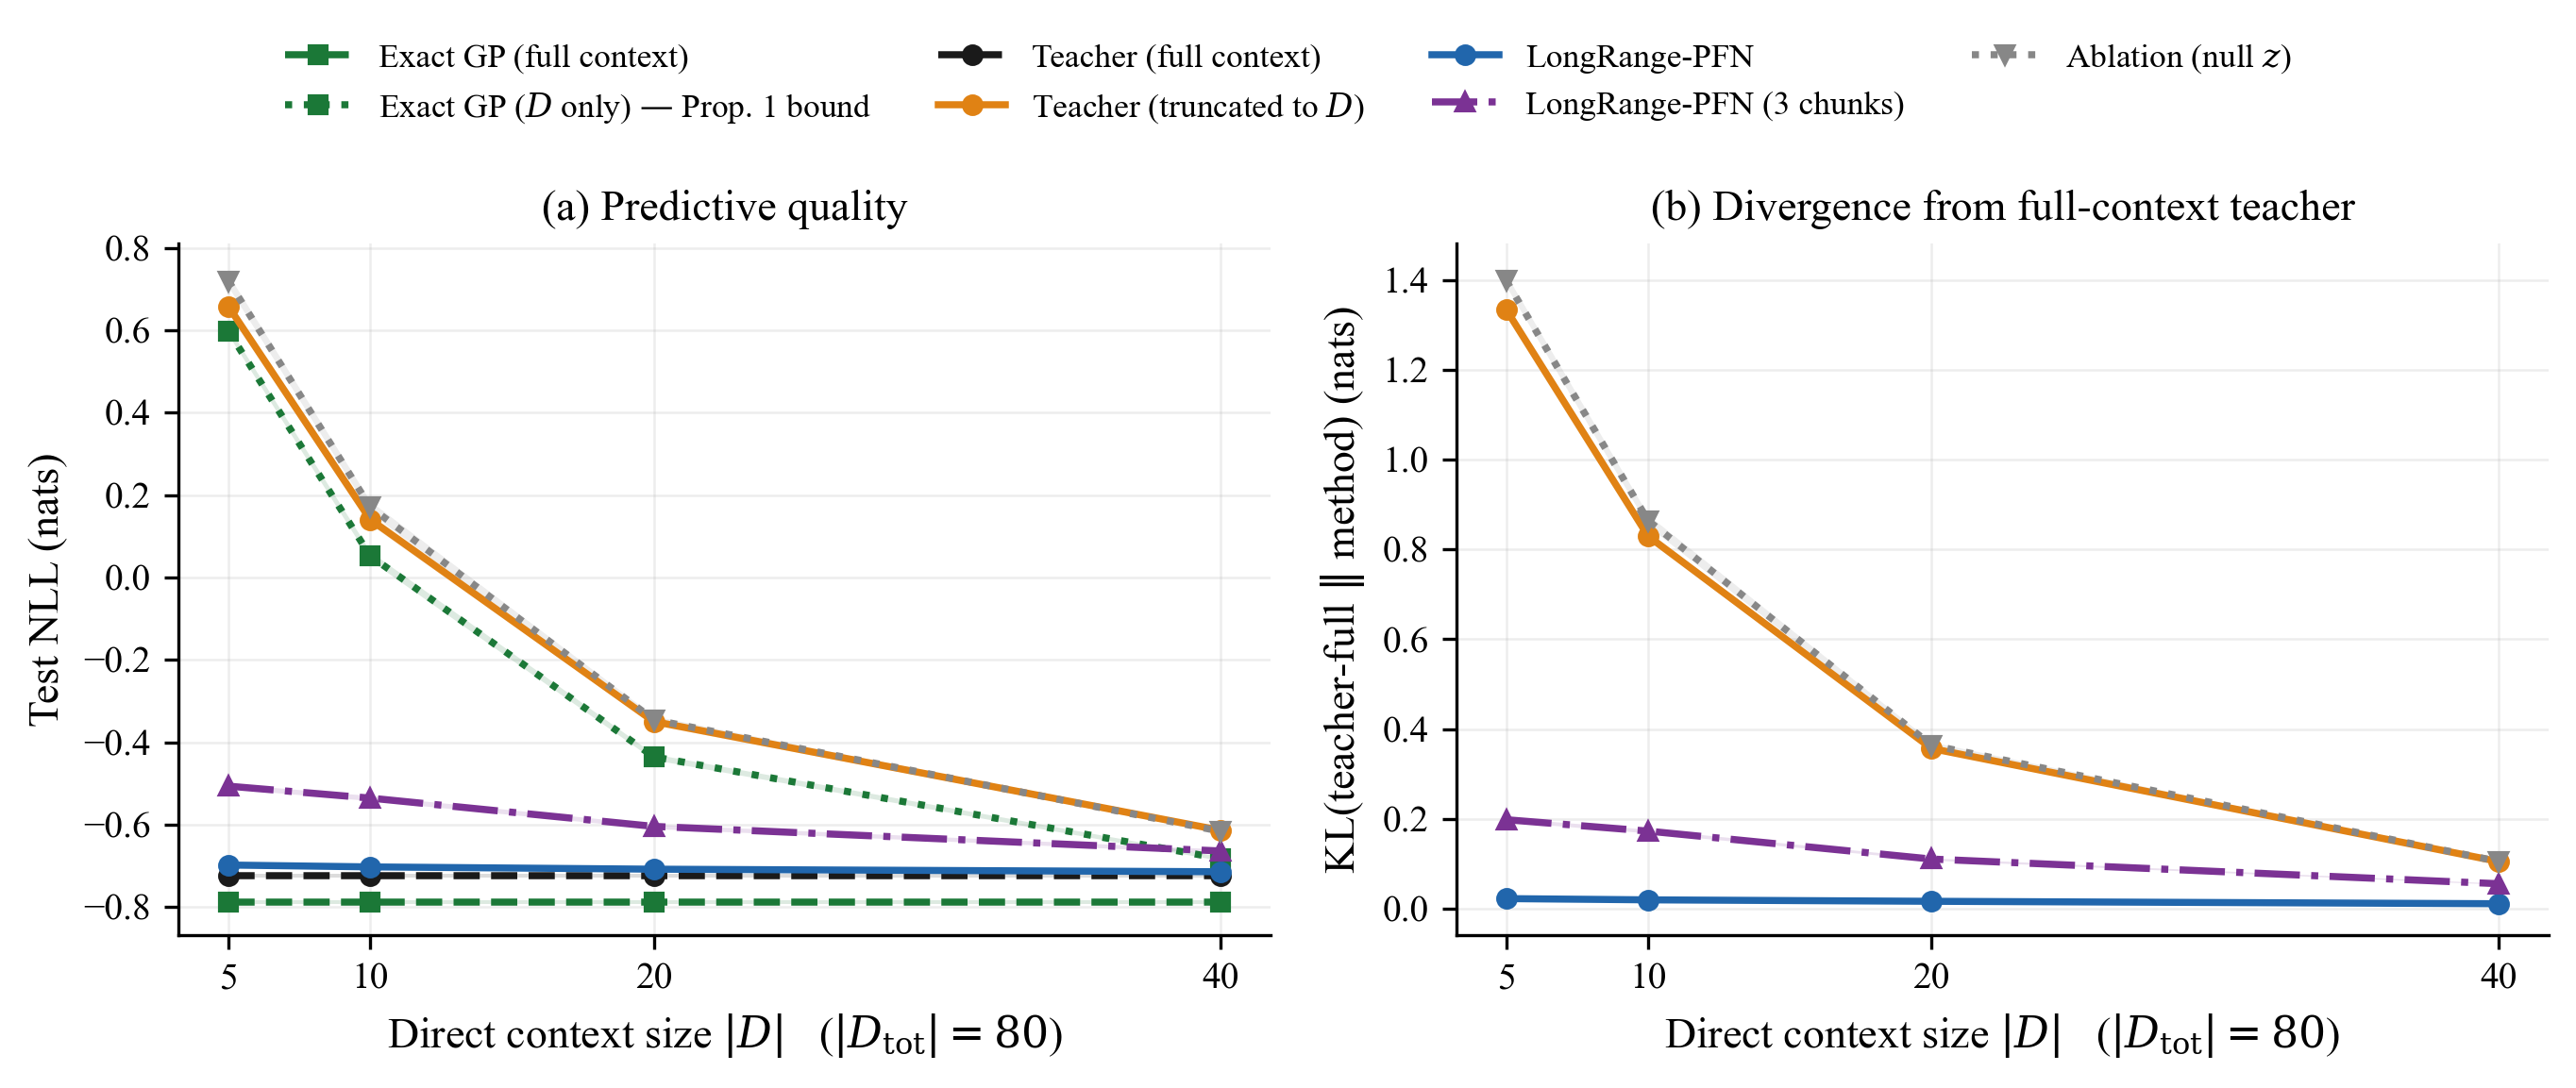
\includegraphics[width=\linewidth]{../results/sweep.png}
\caption{\textbf{Closing the truncation gap} (mean $\pm$ 95\% CI, $3{,}200$ data
sets). (a)~Test NLL vs.\ $|\Dloc|$: the single-shot student (blue) tracks the
full-context reference (black, dashed) and stays below the exact-GP-on-$\Dloc$
bound (green, dotted); the 3-chunk variant (purple) trails.
(b)~KL to teacher-full; the no-$z$ ablation (gray) tracks truncation.}
\label{fig:sweep}
\end{figure}

\begin{figure}[htbp]
\centering
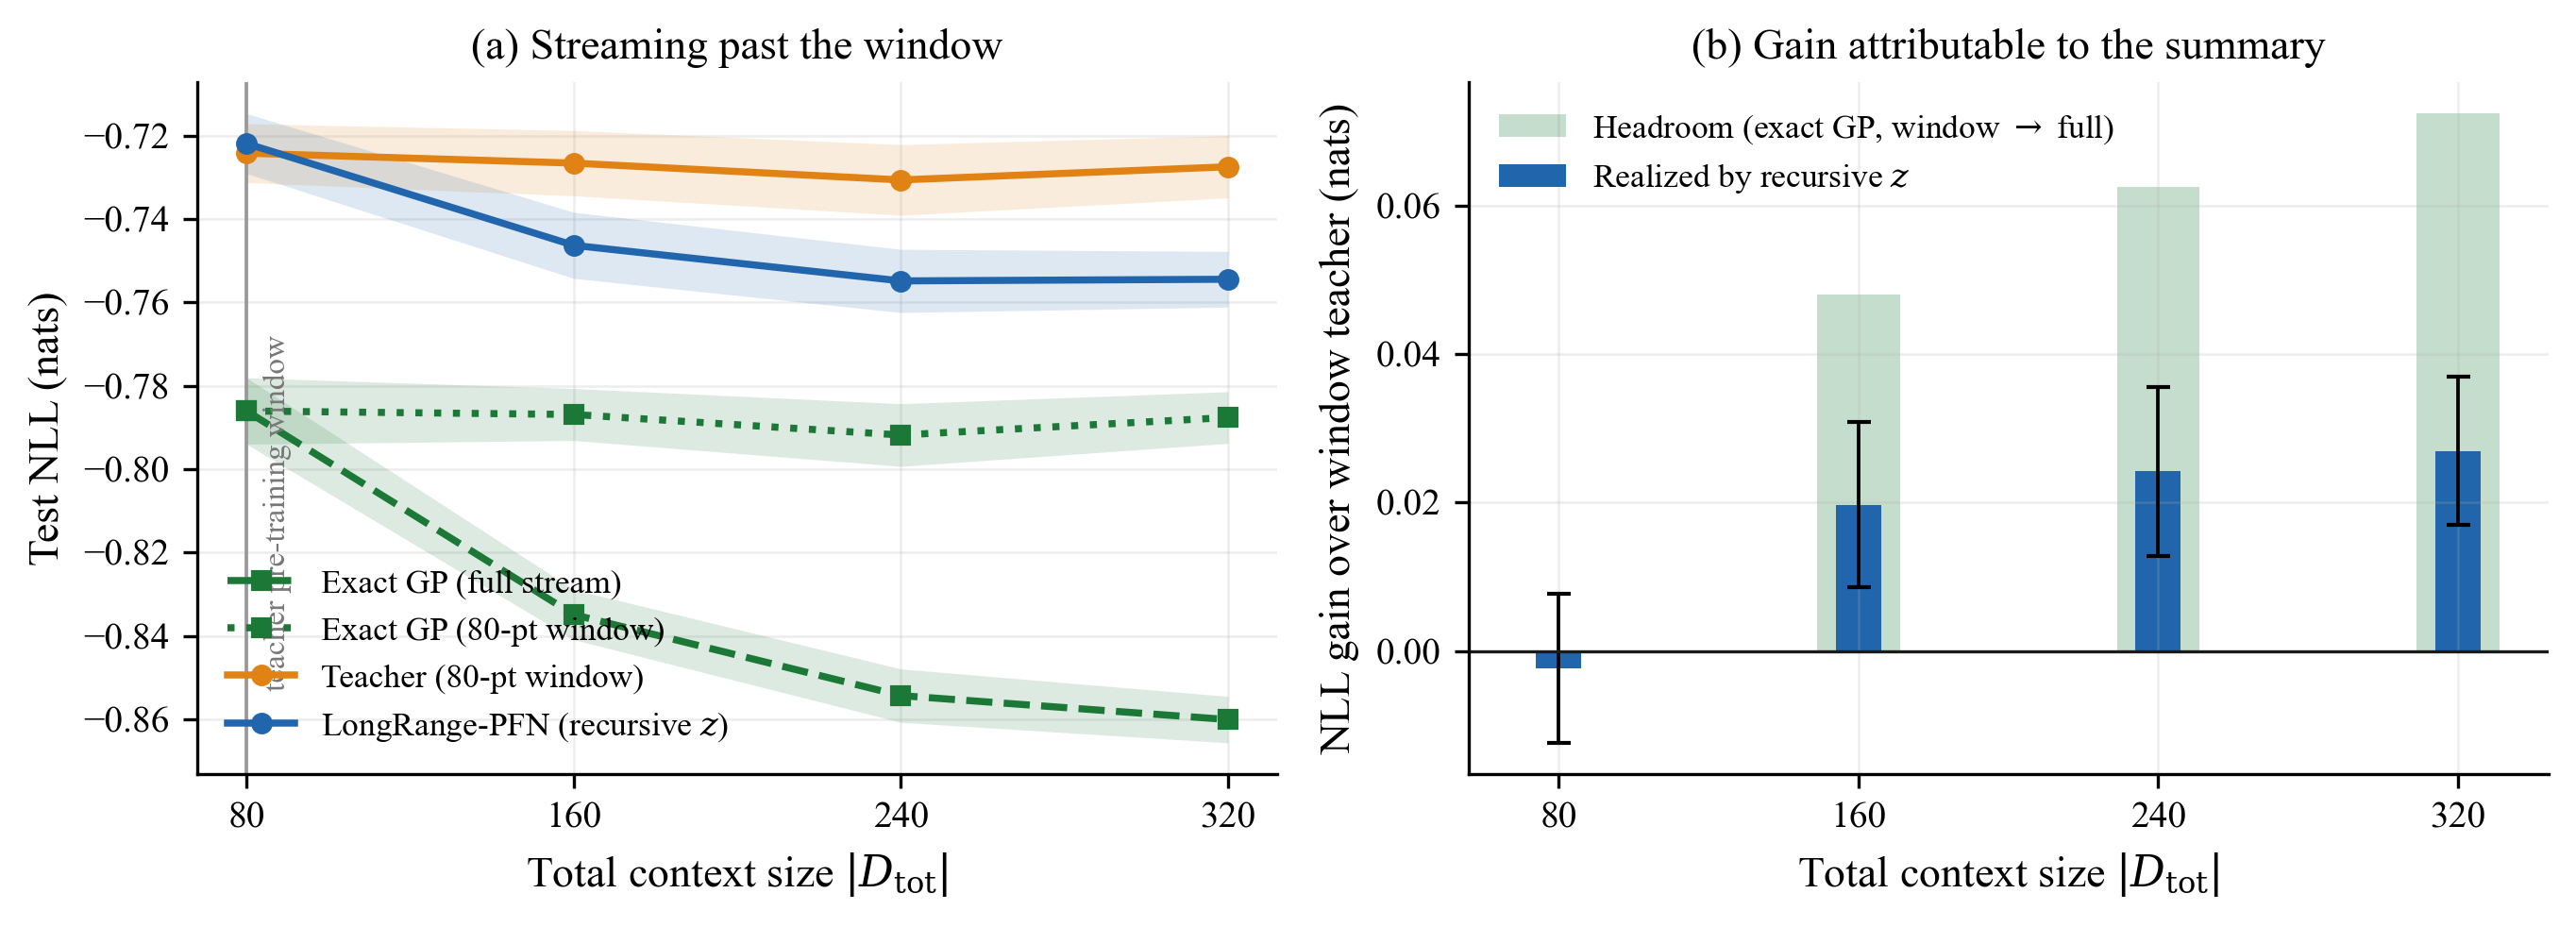
\includegraphics[width=\linewidth]{../results/beyond_window.png}
\caption{\textbf{Streaming beyond the window} (mean $\pm$ 95\% CI, $1{,}280$
data sets). (a)~Test NLL vs.\ total context size: the window teacher (orange) is
flat, the exact GP on the full stream (green, dashed) improves with evidence,
and the recursive student (blue) surpasses the teacher as the stream grows.
(b)~Gain over the window teacher (blue) against the headroom to the full exact
posterior (green).}
\label{fig:beyond}
\end{figure}

\begin{figure}[htbp]
\centering
\begin{minipage}[t]{0.48\linewidth}
\centering
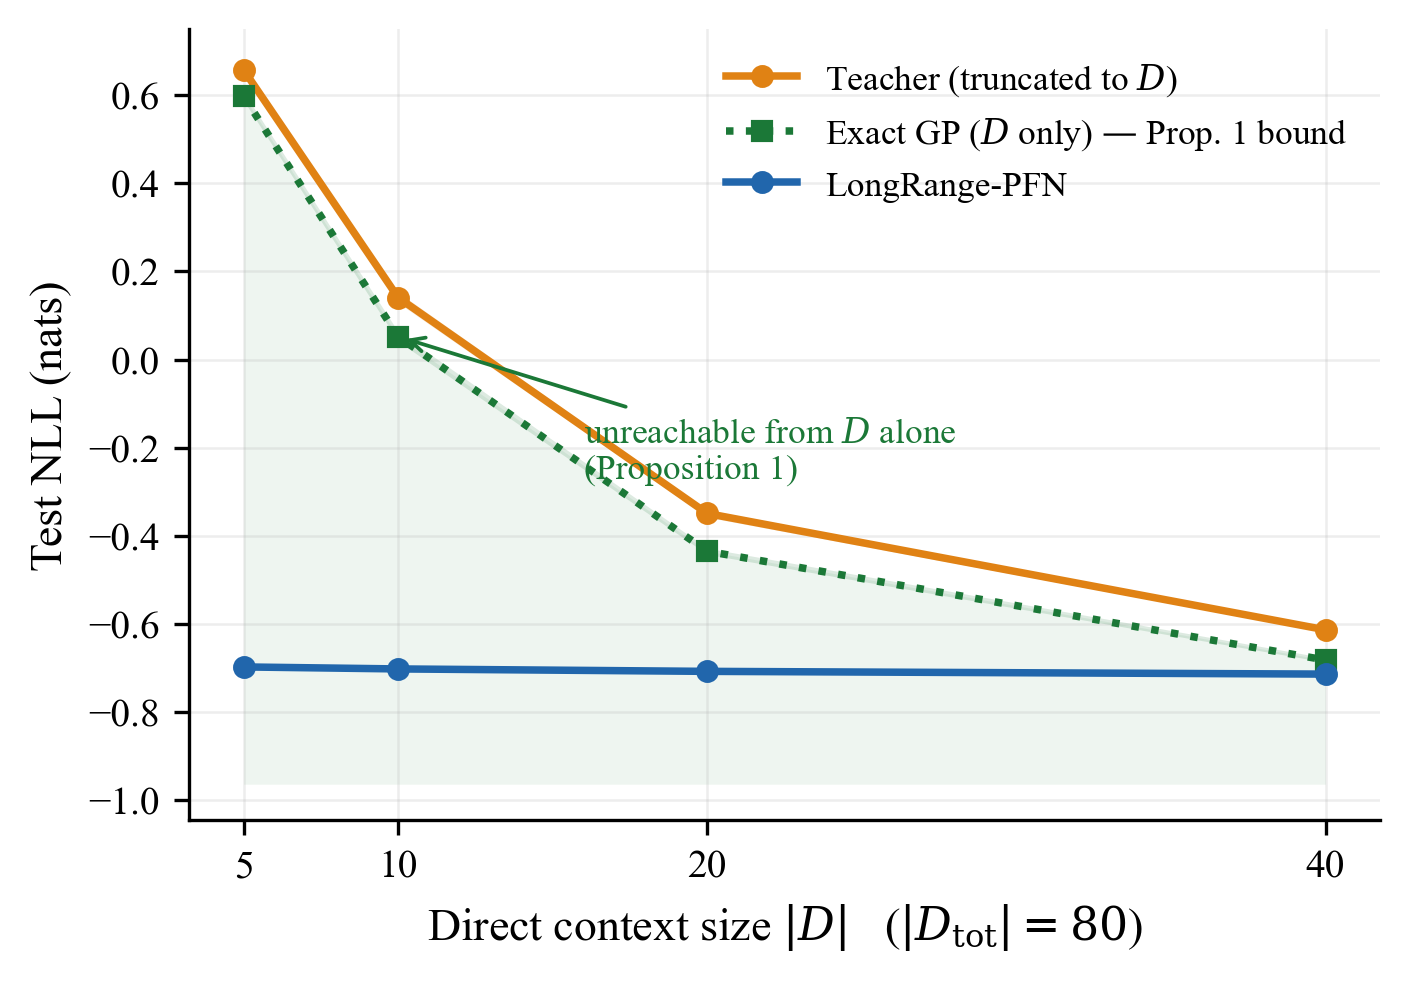
\includegraphics[width=\linewidth]{../results/certificate.png}
\caption{\textbf{The Proposition~\ref{prop:bound} certificate.} The exact GP on
$\Dloc$ (green, dotted) lower-bounds any $\Dloc$-only method; the shaded region
is unreachable without outside information. The student (blue) sits inside it at
every $|\Dloc|$.}
\label{fig:certificate}
\end{minipage}\hfill
\begin{minipage}[t]{0.48\linewidth}
\centering
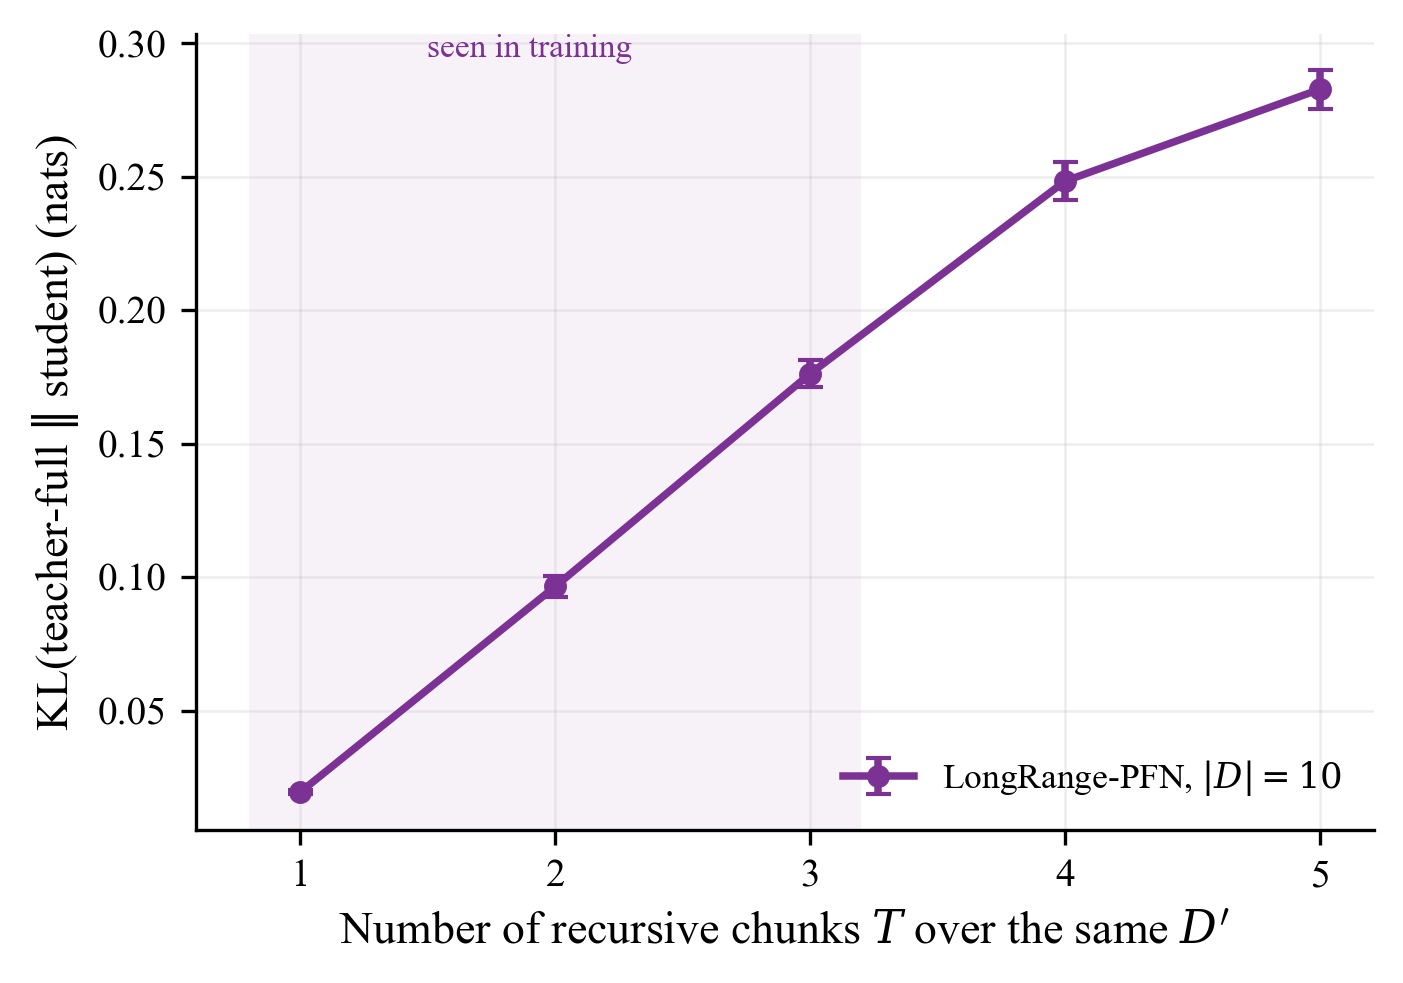
\includegraphics[width=\linewidth]{../results/chunks.png}
\caption{\textbf{Recursion cost.} KL to teacher-full when the same $\Dfar$
($|\Dfar|=70$, $|\Dloc|=10$) is folded in $T$ chunks: \chunkonekl{} nats at
$T=1$ to \chunkfivekl{} nats at $T=5$. Shaded: training range ($T\le 3$). Traced
to a validation criterion that only checks $T=1$
(Appendix~\ref{app:training}).}
\label{fig:chunks}
\end{minipage}
\end{figure}

\begin{figure}[htbp]
\centering
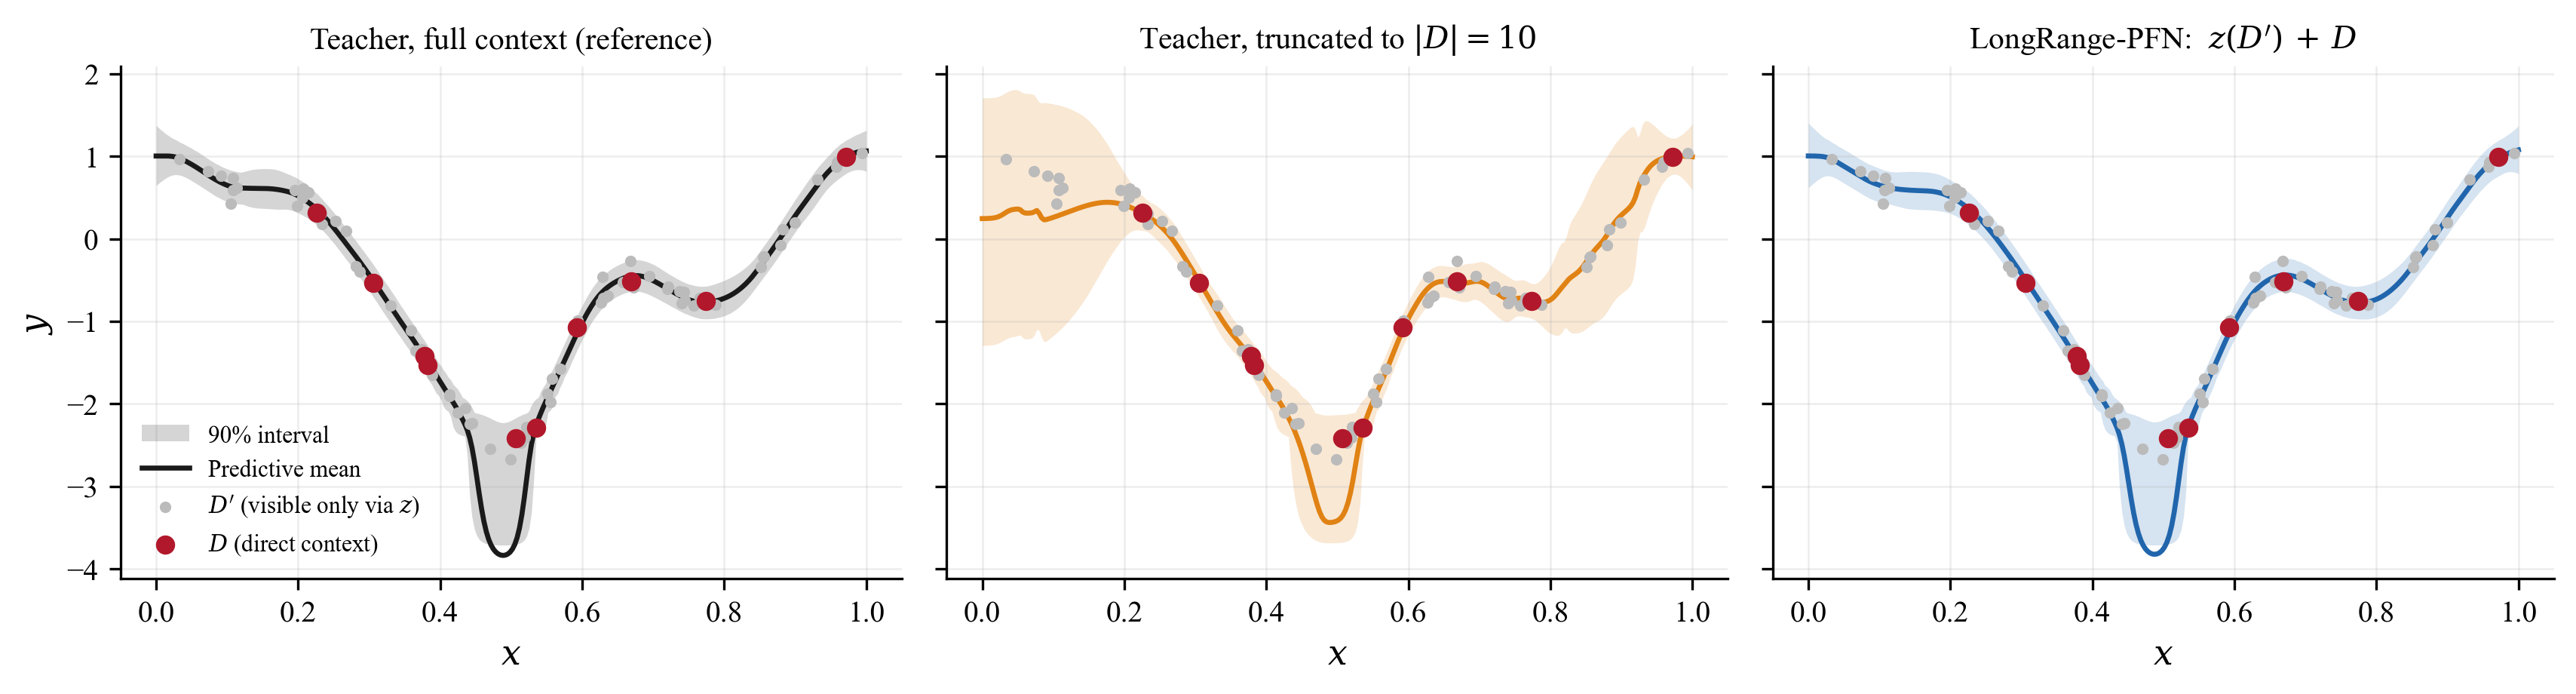
\includegraphics[width=\linewidth]{../results/qualitative.png}
\caption{\textbf{Qualitative behaviour} on one GP draw ($|\Dloc|=10$, red;
$\Dfar$, gray, visible to the student only through $z$). Predictive mean and
90\% interval. The truncated PFN (middle) is overdispersed away from $\Dloc$;
LongRange-PFN (right) sharpens toward the full-context predictive (left) using
$z$ alone.}
\label{fig:qual}
\end{figure}

\paragraph{Calibration and where the summary helps.} Coverage of central
predictive intervals at $|\Dloc|=10$ (Figure~\ref{fig:diagnostics}, left) shows
the student's reliability curve closest to the diagonal, with truncation
under-covering and teacher-full mildly conservative, consistent with the
forward KL preserving the teacher's uncertainty. Binning test points by distance
to the nearest point of $\Dloc$ (right) shows the student's gain over truncation
growing with distance and vanishing near $\Dloc$, the spatial signature of the
certificate. A linear probe of $z$ (Appendix~\ref{app:probe}) decodes the
full-context predictive mean from $\mathrm{vec}(z)$ across the domain (held-out
$R^2 \in [0.3, 0.9]$), so $z$ encodes the function rather than memorizing
points.

\begin{figure}[htbp]
\centering
\begin{minipage}[t]{0.48\linewidth}
\centering
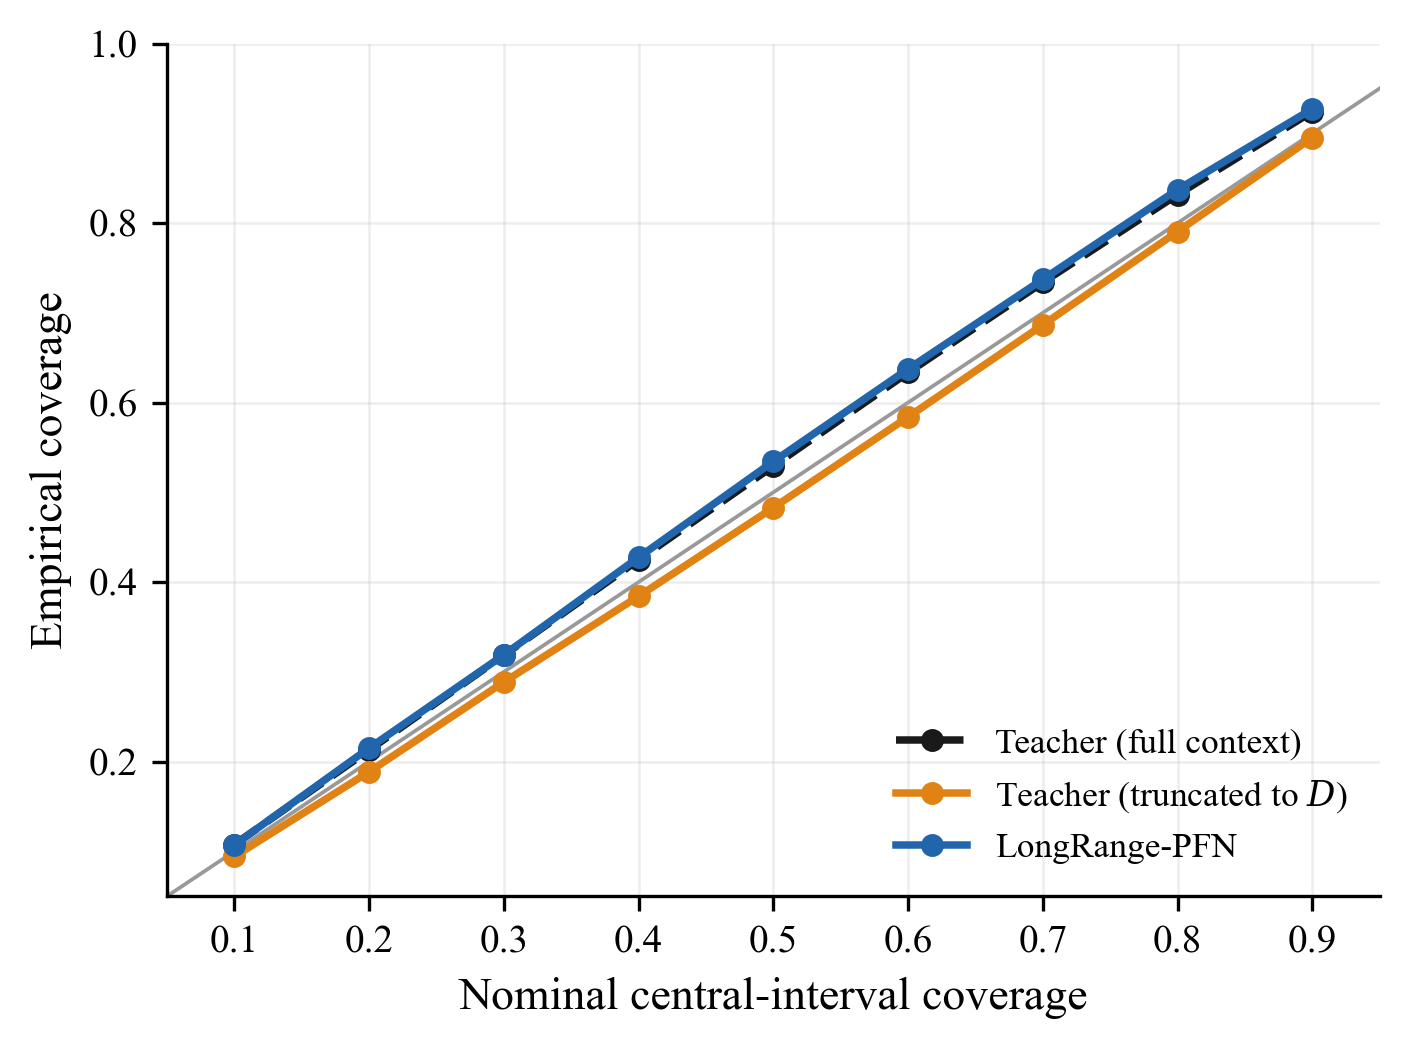
\includegraphics[width=\linewidth]{../results/calibration.png}
\end{minipage}\hfill
\begin{minipage}[t]{0.48\linewidth}
\centering
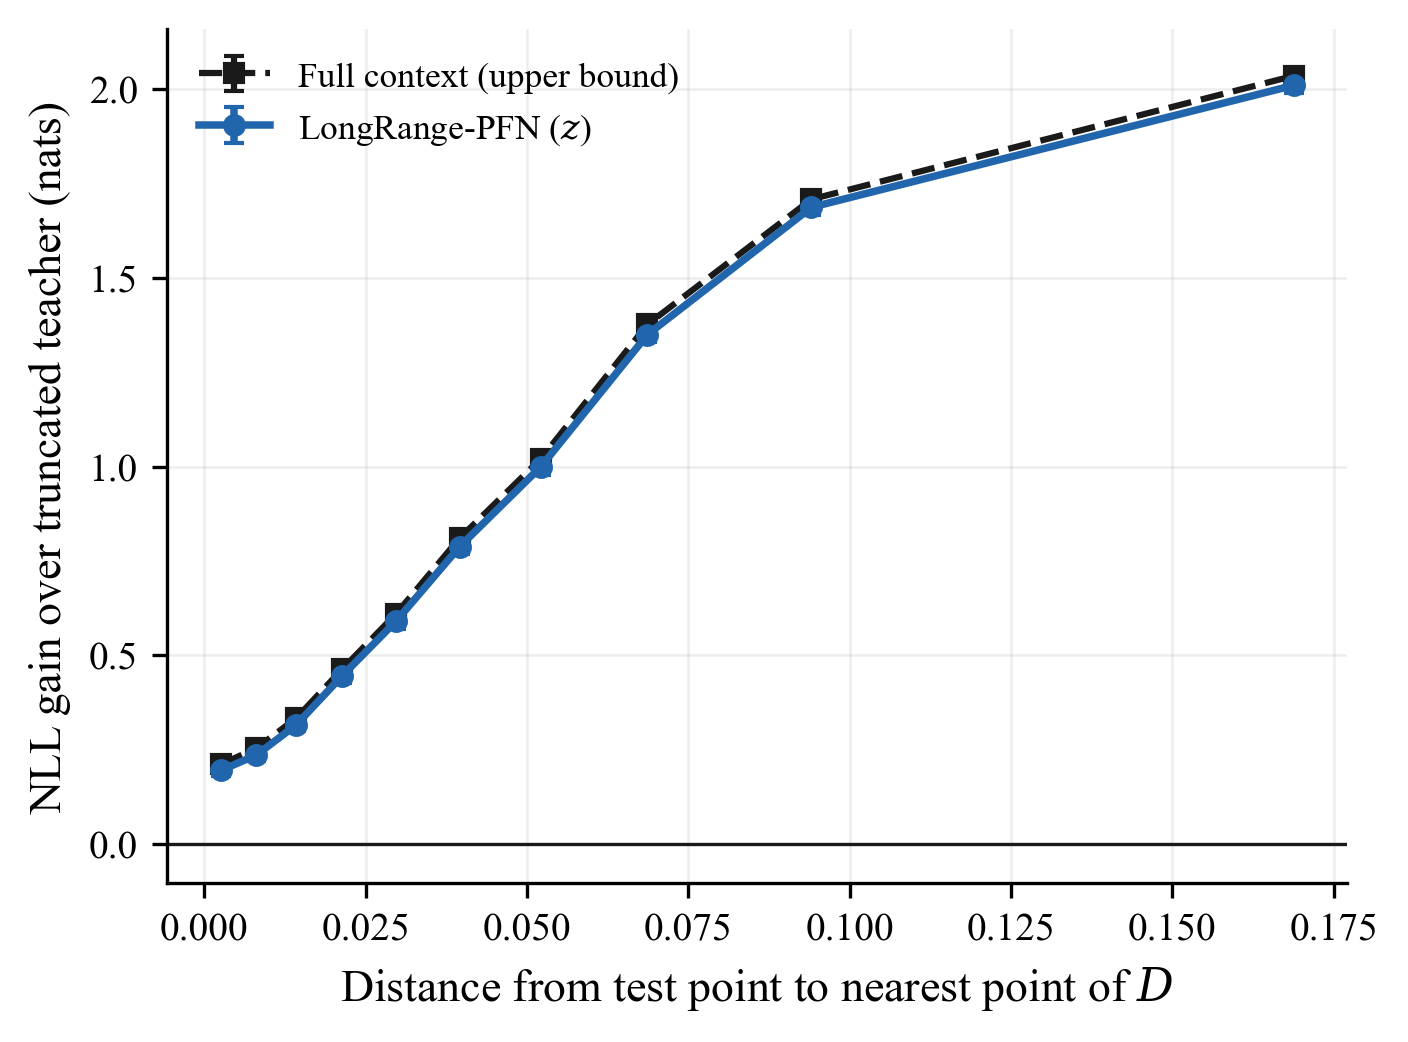
\includegraphics[width=\linewidth]{../results/where_it_helps.png}
\end{minipage}
\caption{\textbf{Diagnostics at $|\Dloc| = 10$.} Left: coverage of central
predictive intervals; the student (blue) is closest to the diagonal. Right: NLL
gain over teacher-local, binned by distance to the nearest point of $\Dloc$; the
gain grows with distance and stays below the full-context ceiling (dashed).}
\label{fig:diagnostics}
\end{figure}

\section{Limitations}
\label{sec:limitations}

This is a proof of concept on a 1-d GP prior with a small teacher and
exchangeable contexts. Chunk order does not matter here but would under
non-stationary data, where the recursion should be a proper filter. The summary
size $k$ is an information bottleneck we have not characterized as a
rate--distortion trade-off. The distillation ceiling is the teacher's own
quality within its window; past that the recursion is validated only
empirically. Checkpoint selection is a concrete gap: the validation set only
checked single-chunk quality, so the selected checkpoint is good at $T=1$ and
worse at higher $T$ (Figure~\ref{fig:chunks}), a cheap fix we have not made.
Finally, Appendix~\ref{app:baselines} shows a fitted classical GP or
full-context TabPFN still beat bounded-state inference here, because exact
inference on this prior is cheap. A real advantage needs a prior where exact
inference is intractable, a teacher at TabPFN's scale, query-aware summaries
$z(x)$, and the associativity regularizer of Section~\ref{sec:recursive}.

\section{Conclusion}

LongRange-PFN carries out-of-window evidence in a few latent tokens, trained
only by distilling a frozen teacher's predictive distribution. On GP priors the
summary provably carries posterior information, crossing the exact lower bound
of Proposition~\ref{prop:bound} at every context size tested, and the recursive
update handles streams four times the training window at constant state while
beating a strong recency baseline. Two gaps remain, both concrete and
measurable: multi-chunk summarization lags single-shot because our validation
set never checked it, and bounded-state inference still trails classical
full-context methods on this easy prior.

\section*{Reproducibility statement}

All code (built on the official PFN repository), training scripts, seeds and
configurations, and the scripts that regenerate every number, table and figure
from \texttt{results/metrics.json} are in the accompanying repository.

\appendix

\section{Training curves}
\label{app:training}

Figure~\ref{fig:training} shows the optimization traces for both stages. Every
regime flattens well before the final step, which is why we select the reported
checkpoint by validation KL rather than by step count, and why the
single-shot-only validation set leaves multi-chunk quality unoptimized.

\begin{figure}[htbp]
\centering
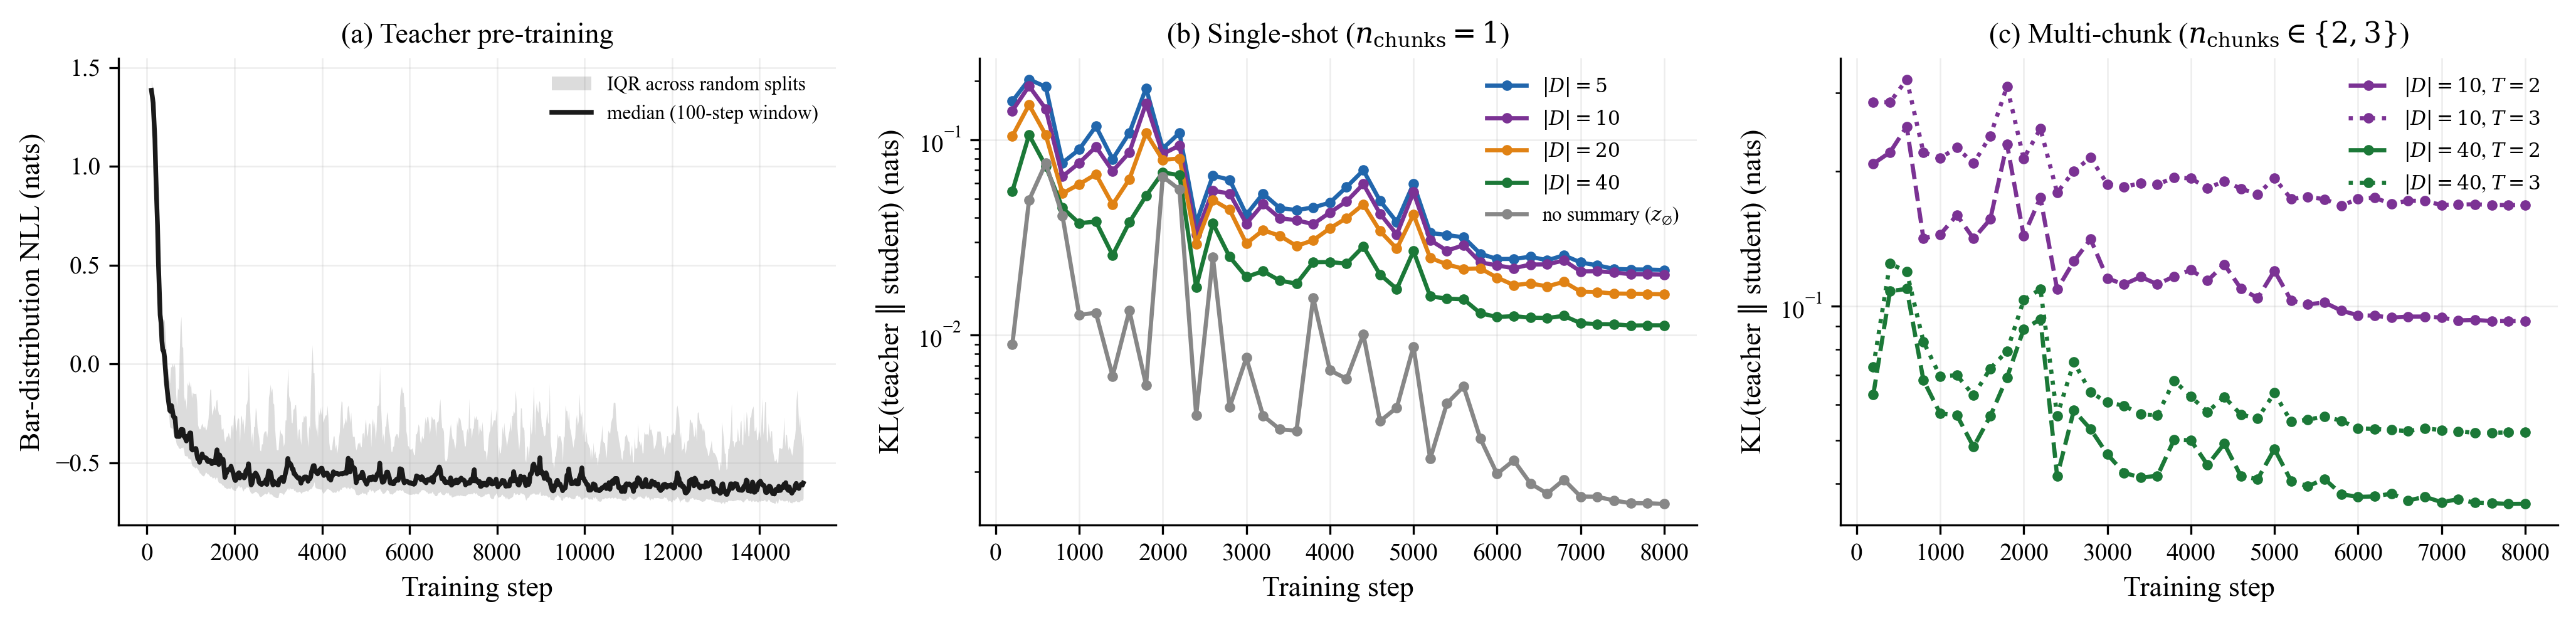
\includegraphics[width=\linewidth]{../results/training_curves.png}
\caption{\textbf{Optimization traces.} (a)~Teacher pre-training:
bar-distribution NLL (rolling median, solid; IQR, shaded). (b)~Student
distillation: validation KL(teacher $\Vert$ student), one line per $|\Dloc|$
regime. Every regime flattens by step $\sim\!12{,}000$, so we select by
validation KL rather than final step. This validation set only covers
single-shot summarization, which is why the checkpoint is strong at $T=1$ and
worse at higher $T$ (Figure~\ref{fig:chunks}).}
\label{fig:training}
\end{figure}

\section{Defensive baselines at large context}
\label{app:baselines}

The main text asks whether the summary preserves information truncation
destroys. A harder question: why not give all the data to a method with no
window? TabPFN, a fitted GP, and a random forest have no $80$-point limit, so
here we give them the entire context, up to $8\times$ the teacher's window, and
check whether LongRange-PFN, a recent local window plus an $O(k)$ recursive
summary, holds up.

Table~\ref{tab:baselines} covers $N \in \{80, 160, 320, 640\}$ using an earlier
teacher/student pair trained with a shorter schedule; the conclusion follows
from the prior being easy for a matched kernel, not from the checkpoint, but we
flag the mismatch. Full-context baselines are TabPFN
\citep{hollmann2025tabpfn}, a scikit-learn GP with an RBF kernel fit per data
set (unlike the ``GP exact'' oracle, which uses the true hyperparameters),
kernel ridge, $k$-NN, and a random forest, all given the full $N$ points;
LongRange-PFN and the recency teacher see only bounded state.

A fitted RBF GP ends up close to the oracle, unsurprising since the data come
from an RBF GP, and full-context TabPFN is also strong; both beat the
bounded-state methods in NLL by $0.1$--$0.2$ nats. This is an easy
point-prediction task for a matched kernel, so it was never going to show a
predictive win over classical methods. That is fine: the contribution is not a
better predictor on GP data, where exact inference is cheap, but a
bounded-state mechanism for carrying evidence when the full context cannot be
stored and re-attended. A predictive win over strong full-data baselines would
need a prior where exact inference is intractable and a teacher at TabPFN's
scale.

\begin{table}[htbp]
\centering
\caption{Large-context defensive baselines over total context size $N$ (up to
$8\times$ the teacher's window; $100$ data sets per cell, TabPFN on its own
smaller sample). \emph{Full-context} baselines see all $N$ points;
\emph{bounded-state} methods see only recent points plus, for LongRange-PFN, the
$O(k)$ summary. NLL (nats) for probabilistic methods, RMSE for all; mean $\pm$
s.e.}
\label{tab:baselines}
\resizebox{\textwidth}{!}{\begin{tabular}{lcccc}
\toprule
\multicolumn{5}{c}{\emph{NLL (nats, lower is better)}}\\
\midrule
Method & $N=80$ & $N=160$ & $N=320$ & $N=640$\\
\midrule
Teacher (80-pt window) & -0.693\,{\scriptsize$\pm$0.016} & -0.682\,{\scriptsize$\pm$0.015} & -0.697\,{\scriptsize$\pm$0.014} & -0.716\,{\scriptsize$\pm$0.014}\\
\textbf{LongRange-PFN (bounded)} & -0.678\,{\scriptsize$\pm$0.016} & -0.662\,{\scriptsize$\pm$0.014} & -0.684\,{\scriptsize$\pm$0.014} & -0.702\,{\scriptsize$\pm$0.012}\\
GP exact (full, oracle) & -0.789\,{\scriptsize$\pm$0.012} & -0.824\,{\scriptsize$\pm$0.011} & -0.859\,{\scriptsize$\pm$0.011} & -0.893\,{\scriptsize$\pm$0.010}\\
TabPFN (full context) & -0.632\,{\scriptsize$\pm$0.024} & -0.723\,{\scriptsize$\pm$0.020} & -0.782\,{\scriptsize$\pm$0.020} & -0.756\,{\scriptsize$\pm$0.024}\\
GP-RBF fitted (full) & -0.771\,{\scriptsize$\pm$0.014} & -0.815\,{\scriptsize$\pm$0.011} & -0.856\,{\scriptsize$\pm$0.011} & -0.891\,{\scriptsize$\pm$0.011}\\
\midrule
\multicolumn{5}{c}{\emph{RMSE (lower is better)}}\\
\midrule
Method & $N=80$ & $N=160$ & $N=320$ & $N=640$\\
\midrule
Teacher (80-pt window) & 0.142\,{\scriptsize$\pm$0.008} & 0.154\,{\scriptsize$\pm$0.009} & 0.148\,{\scriptsize$\pm$0.009} & 0.140\,{\scriptsize$\pm$0.008}\\
\textbf{LongRange-PFN (bounded)} & 0.141\,{\scriptsize$\pm$0.008} & 0.153\,{\scriptsize$\pm$0.008} & 0.147\,{\scriptsize$\pm$0.009} & 0.139\,{\scriptsize$\pm$0.008}\\
GP exact (full, oracle) & -- & -- & -- & --\\
TabPFN (full context) & 0.120\,{\scriptsize$\pm$0.004} & 0.106\,{\scriptsize$\pm$0.002} & 0.103\,{\scriptsize$\pm$0.002} & 0.101\,{\scriptsize$\pm$0.002}\\
GP-RBF fitted (full) & 0.111\,{\scriptsize$\pm$0.002} & 0.106\,{\scriptsize$\pm$0.001} & 0.102\,{\scriptsize$\pm$0.001} & 0.099\,{\scriptsize$\pm$0.001}\\
Kernel ridge (full) & 0.110\,{\scriptsize$\pm$0.002} & 0.106\,{\scriptsize$\pm$0.001} & 0.102\,{\scriptsize$\pm$0.001} & 0.098\,{\scriptsize$\pm$0.001}\\
$k$-NN (full) & 0.164\,{\scriptsize$\pm$0.004} & 0.125\,{\scriptsize$\pm$0.002} & 0.113\,{\scriptsize$\pm$0.001} & 0.109\,{\scriptsize$\pm$0.001}\\
Random forest (full) & 0.142\,{\scriptsize$\pm$0.003} & 0.127\,{\scriptsize$\pm$0.002} & 0.123\,{\scriptsize$\pm$0.001} & 0.121\,{\scriptsize$\pm$0.001}\\
\bottomrule
\end{tabular}
}
\end{table}

\section{What does the summary encode?}
\label{app:probe}

We probe what information the latent $z$ carries with a ridge decoder from
$\mathrm{vec}(z)$ to the full-context predictive mean and a PCA of the summary
space (Figure~\ref{fig:probe}).

\begin{figure}[htbp]
\centering
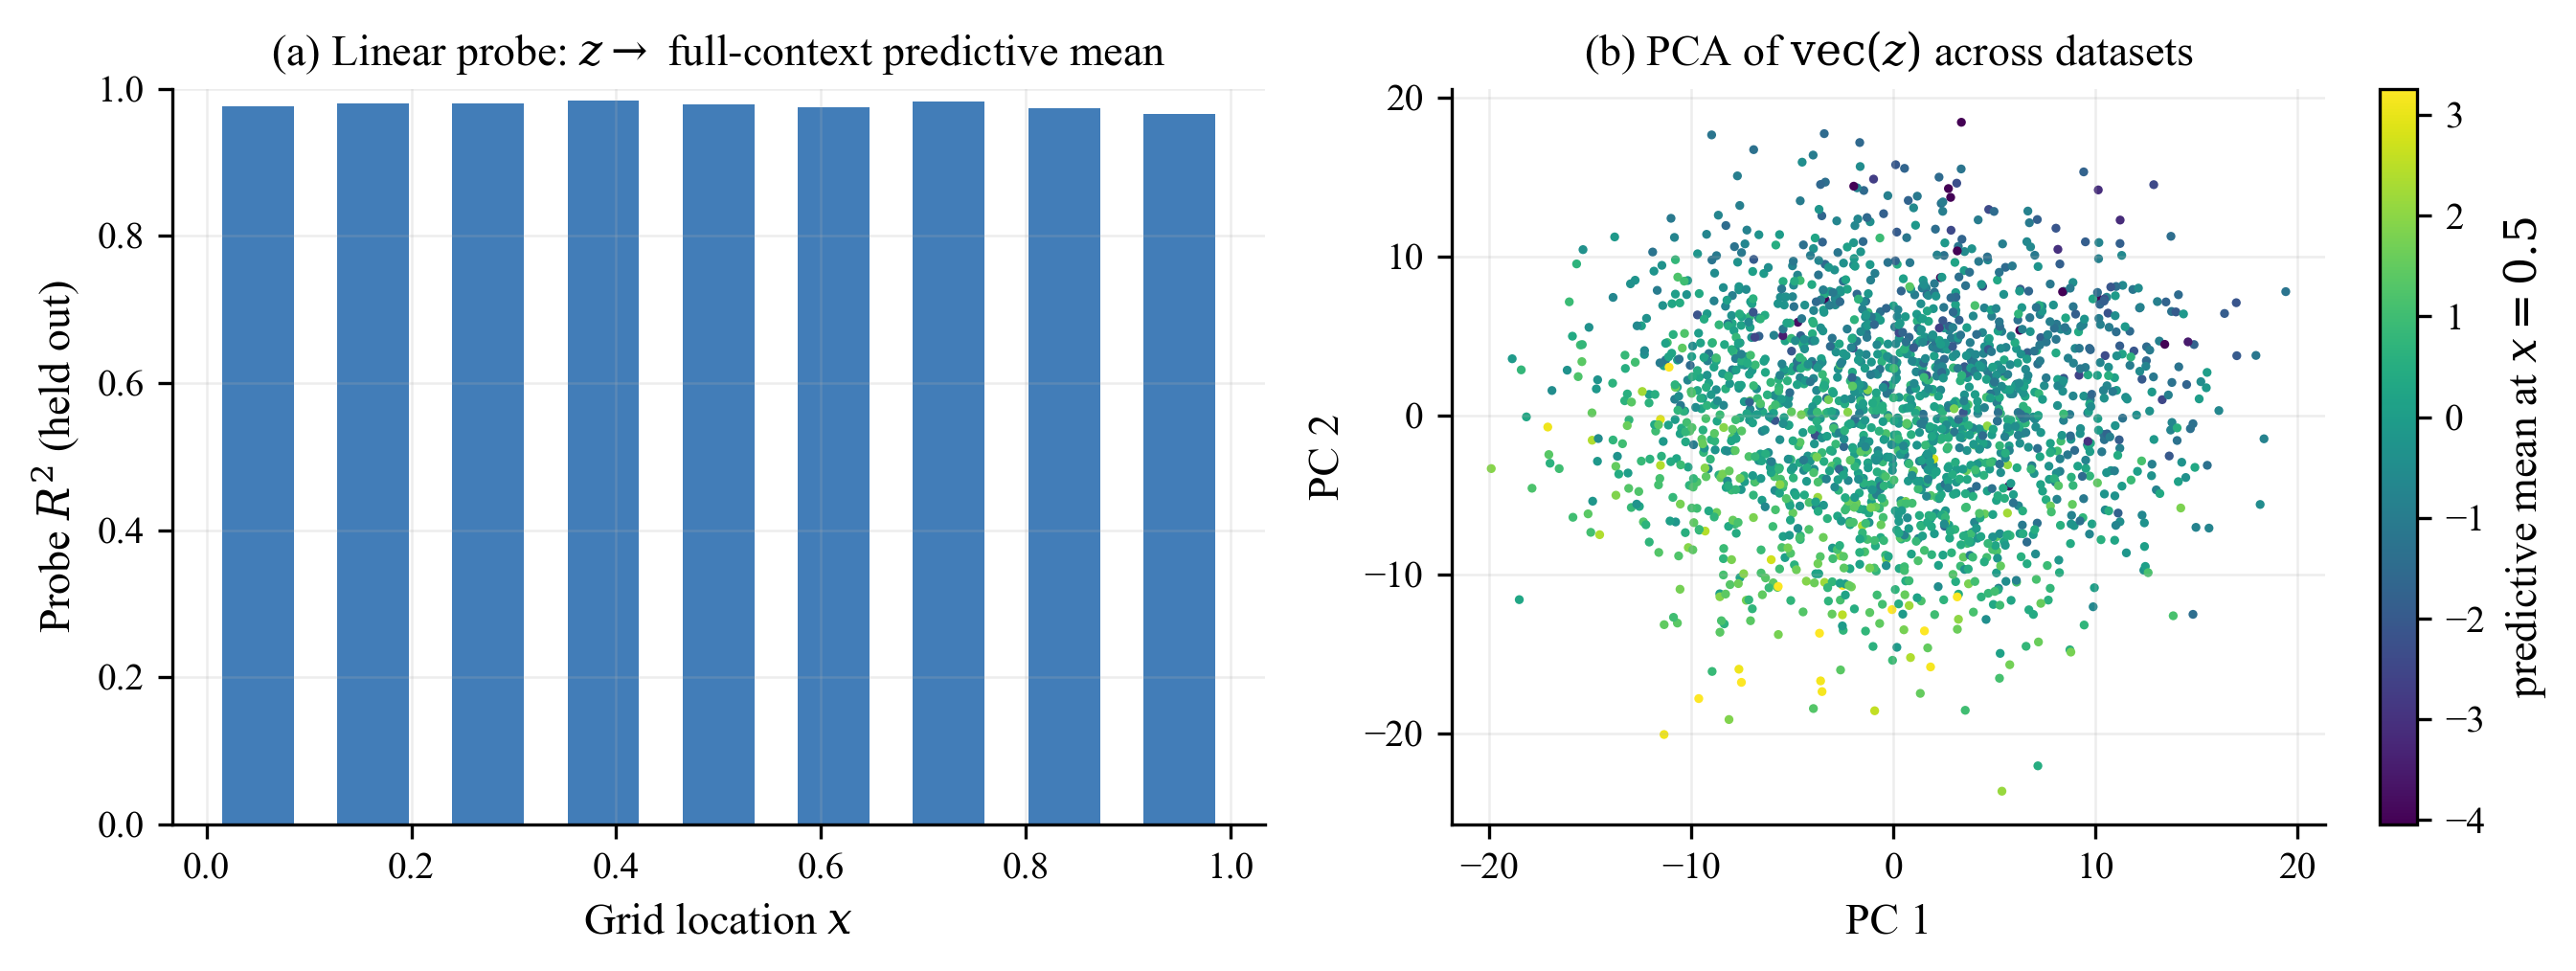
\includegraphics[width=\linewidth]{../results/latent_probe.png}
\caption{\textbf{Probing the summary space} ($z$ from all $80$ context points;
$\approx 1{,}900$ held-out data sets). (a)~Held-out $R^2$ of a ridge probe from
$\mathrm{vec}(z)$ to the full-context teacher's predictive mean at each grid
location: partially decodable everywhere ($R^2 \approx 0.3$ mid-domain to
$0.9$ near the boundary). (b)~First two principal components of
$\mathrm{vec}(z)$, colored by the predictive mean at $x=0.5$: the space is
coarsely organized by function value.}
\label{fig:probe}
\end{figure}

\begin{thebibliography}{18}

\bibitem[M\"uller et al.(2022)]{muller2022pfn}
S.~M\"uller, N.~Hollmann, S.~Pineda-Arango, J.~Grabocka, F.~Hutter.
\newblock Transformers Can Do Bayesian Inference.
\newblock \emph{ICLR}, 2022.

\bibitem[Hollmann et al.(2023)]{hollmann2023tabpfn}
N.~Hollmann, S.~M\"uller, K.~Eggensperger, F.~Hutter.
\newblock TabPFN: A Transformer That Solves Small Tabular Classification
Problems in a Second.
\newblock \emph{ICLR}, 2023.

\bibitem[Hollmann et al.(2025)]{hollmann2025tabpfn}
N.~Hollmann, S.~M\"uller, L.~Purucker, A.~Krishnakumar, M.~K\"orfer,
S.~B.~Hoo, R.~T.~Schirrmeister, F.~Hutter.
\newblock Accurate predictions on small data with a tabular foundation model.
\newblock \emph{Nature}, 637:319--326, 2025.

\bibitem[Feuer et al.(2024)]{feuer2024tunetables}
B.~Feuer, R.~T.~Schirrmeister, V.~Cherepanova, C.~Hegde, F.~Hutter,
M.~Goldblum, N.~Cohen, C.~White.
\newblock TuneTables: Context Optimization for Scalable Prior-Data Fitted
Networks.
\newblock \emph{NeurIPS}, 2024.

\bibitem[Ma et al.(2024)]{ma2024icd}
J.~Ma, V.~Thomas, G.~Yu, A.~Caterini.
\newblock In-Context Data Distillation with TabPFN.
\newblock \emph{arXiv:2402.06971}, 2024.

\bibitem[Thomas et al.(2024)]{thomas2024localpfn}
V.~Thomas, J.~Ma, R.~Hosseinzadeh, K.~Golestan, G.~Yu, M.~Volkovs,
A.~Caterini.
\newblock Retrieval \& Fine-Tuning for In-Context Tabular Models.
\newblock \emph{NeurIPS}, 2024.

\bibitem[Heredge et al.(2026)]{heredge2026crumb}
J.~Heredge, M.~J.~Villani, P.~Deshpande, A.~Seshadri, N.~Kumar.
\newblock CRUMB: Efficient Prior Fitted Network Inference via Distributionally
Matched Context Batching.
\newblock \emph{arXiv:2606.11473}, 2026.

\bibitem[Mu et al.(2023)]{mu2023gisting}
J.~Mu, X.~L.~Li, N.~Goodman.
\newblock Learning to Compress Prompts with Gist Tokens.
\newblock \emph{NeurIPS}, 2023.

\bibitem[Ge et al.(2024)]{ge2023icae}
T.~Ge, J.~Hu, L.~Wang, X.~Wang, S.-Q.~Chen, F.~Wei.
\newblock In-context Autoencoder for Context Compression in a Large Language
Model.
\newblock \emph{ICLR}, 2024.

\bibitem[Chevalier et al.(2023)]{chevalier2023autocompressors}
A.~Chevalier, A.~Wettig, A.~Ajith, D.~Chen.
\newblock Adapting Language Models to Compress Contexts.
\newblock \emph{EMNLP}, 2023.

\bibitem[Bulatov et al.(2022)]{bulatov2022rmt}
A.~Bulatov, Y.~Kuratov, M.~Burtsev.
\newblock Recurrent Memory Transformer.
\newblock \emph{NeurIPS}, 2022.

\bibitem[Garnelo et al.(2018)]{garnelo2018np}
M.~Garnelo, J.~Schwarz, D.~Rosenbaum, F.~Viola, D.~J.~Rezende,
S.~M.~A.~Eslami, Y.~W.~Teh.
\newblock Neural Processes.
\newblock \emph{ICML Workshop on Theoretical Foundations and Applications of
Deep Generative Models}, 2018.

\bibitem[Kim et al.(2019)]{kim2019anp}
H.~Kim, A.~Mnih, J.~Schwarz, M.~Garnelo, A.~Eslami, D.~Rosenbaum,
O.~Vinyals, Y.~W.~Teh.
\newblock Attentive Neural Processes.
\newblock \emph{ICLR}, 2019.

\bibitem[Chen et al.(2021)]{chen2021nass}
Y.~Chen, D.~Zhang, M.~U.~Gutmann, A.~Courville, Z.~Zhu.
\newblock Neural Approximate Sufficient Statistics for Implicit Models.
\newblock \emph{ICLR}, 2021.

\bibitem[Mittal et al.(2025)]{mittal2025amortized}
S.~Mittal, N.~L.~Bracher, G.~Lajoie, P.~J\"akel, S.~Bauer.
\newblock Amortized In-Context Bayesian Posterior Estimation.
\newblock \emph{arXiv:2502.06601}, 2025.

\bibitem[Hinton et al.(2015)]{hinton2015distillation}
G.~Hinton, O.~Vinyals, J.~Dean.
\newblock Distilling the Knowledge in a Neural Network.
\newblock \emph{NeurIPS Deep Learning Workshop}, 2015.

\bibitem[Korattikara et al.(2015)]{korattikara2015darkknowledge}
A.~Korattikara, V.~Rathod, K.~Murphy, M.~Welling.
\newblock Bayesian Dark Knowledge.
\newblock \emph{NeurIPS}, 2015.

\bibitem[Malinin et al.(2020)]{malinin2020edd}
A.~Malinin, B.~Mlodozeniec, M.~Gales.
\newblock Ensemble Distribution Distillation.
\newblock \emph{ICLR}, 2020.

\end{thebibliography}

\end{document}
